\documentclass[10pt,twocolumn]{article}
\usepackage{times}
\usepackage{multirow}
\usepackage{tabularx}
\usepackage{subcaption}
\usepackage{graphicx,grffile}
\usepackage{pgf}
\usepackage{tikz}
\usetikzlibrary{arrows,automata}
\usepackage[latin1]{inputenc}

% do not change these values
\baselineskip 12pt
\textheight 9in
\textwidth 6.5in
\oddsidemargin 0in
\topmargin 0in
\headheight 0in
\headsep 0in

%\makeatletter
%\def\maxwidth{\ifdim\Gin@nat@width>\linewidth\linewidth\else\Gin@nat@width\fi}
%\def\maxheight{\ifdim\Gin@nat@height>\textheight\textheight\else\Gin@nat@height\fi}
%\makeatother
%% Scale images if necessary, so that they will not overflow the page
%% margins by default, and it is still possible to overwrite the defaults
%% using explicit options in \includegraphics[width, height, ...]{}
%\setkeys{Gin}{width=\maxwidth,height=\maxheight,keepaspectratio}
%

\usepackage[unicode=true]{hyperref}
\hypersetup{breaklinks=true,
            bookmarks=true,
            pdfauthor={},
            pdftitle={},
            colorlinks=true,
            citecolor=blue,
            urlcolor=blue,
            linkcolor=blue,
            pdfborder={0 0 0}}
\urlstyle{same}  % don't use monospace font for urls

\usepackage[font=footnotesize,labelfont=bf]{caption}

\begin{document}

\title{outline!}

\author{
%Noah Watkins, Neha Ojha\textsuperscript{*}, Carlos Maltzahn \\
%\small {\em University of California, Santa Cruz} \\
%\small {\{jayhawk,carlosm\}@cs.ucsc.edu} \textsuperscript{*}nojha@ucsc.edu \\ [2mm]
\small Submission Type: Research
}

\date{}
\maketitle

\begin{abstract}
To meet the needs of a diverse and growing set of cloud-based applications,
modern distributed storage frameworks expose a variety of composable
subsystems as building blocks.  This approach gives infrastructure programmers
significant flexibility in implementing application-specific semantics while
reusing trusted components.  Unfortunately, in current storage systems the
composition of subsystems is a low-level task that couples (and hence
obscures) a variety of orthogonal concerns, including functional correctness
and performance.  Building an application by wiring together a collection of
components typically requires thousands of lines of carefully-written C++
code, an effort that must be repeated whenever device or subsystem
characteristics change.

In this paper, we propose a declarative approach to subservice composition
that allows programmers to focus on the high-level functional properties that
are required by applications.  Choosing an implementation that is consistent
with the declarative functional specification then can be posed as a search
problem over the space of parameters such as block sizes, storage interfaces
(e.g. key/value or block storage) and concurrency control mechanisms.  We
present experimental evaluation of our prototype, (etc etc)
\end{abstract}

\section{Introduction}

% whats the problem
Storage systems are increasingly providing features that take advantage of
application-specific knowledge to achieve optimizations and provide unique
services. However, this trend is leading to the creation of a large number of
software extensions that will be difficult to maintain as system software and
hardware continue to evolve.

% why is it interesting
The widely deployed Ceph distributed storage system is an example of a storage
system that supports application-specific extensions in the form of custom I/O
interfaces to objects managed by the underlying RADOS object storage
system~\cite{weil:osdi06,weil:pdsw07}. Organizations are increasingly reliant
upon these extensions as is shown in Figure~\ref{fig:objclass-dev} by a marked
increase in the number of object operations that are packaged as part of the
Ceph distribution and widely used by internal Ceph subystems and by
applications such as OpenStack Swift and Cinder~\cite{openstack}. In addition
to the growth in the quantity of operations, Figure~\ref{fig:objclass-dev}
also depicts the amount of low-level C++ written to implement these
operations. Unfortunately, this code is written assuming a performance profile
defined by the combination of the hardware and software versions available at
the time of development. As Ceph continues to evolve at a fast pace, the cost
of adapting application-specific codes to changing assumptions regarding
performance may become significant.

%The construction of object operations is not limited to core Ceph developers;
%the development community has been receptive to contributions with the recent
%inclusion by CERN developers of an extension for performing limited numeric
%operations on object data~\cite{cls_numops}. And while Ceph has not yet
%reached the point of directly exposing these features to non-administrative
%users, the recent inclusion of a mechanism for dynamically defining extensions
%using Lua~\cite{cls_lua} suggests that aspects of this feature may soon appear.


% a challenge is mapping application semantics onto these objects

%Proprietary storage systems are prevalent, but have fixed interfaces that are
%developed in response to market demand. Alternative storage interfaces are
%prototyped in research systems.
%For the first time Ceph is providing a high-performance production quality
%storage system developed as open-source.

% why is it hard / why do naive approaches fail
%the naive approach here is the use of generic interfaces. one may
%think that key-value is relatively slower than bytestreams, but by how much.
%is this a principal we can bet the house on.
%just building these simple interfaces don't work that well
%Systems provide low-level native interfaces such as key-value or bytestream interfaces.
%These abstract interfaces are useful, but they are not the only way to map
%interfaces onto storage. For instance, a specialized key-value db could be serialized into
%the bytestream interface.

\begin{figure}[t]
  \centering
    \includegraphics[width=0.48\textwidth]{experiments/objclass-dev/output.png}
    \caption{
[\href{https://github.com/noahdesu/zlog-popper/tree/master/experiments/objclass-dev/visualize.ipynb}{source}]
Growth of officially supported, custom object interfaces in RADOS over 6
years. An \emph{operation} is a function executed in the context of an object,
and operations are grouped into different \emph{categories}
corresponding to applications or utilities, such as reference counting}
\label{fig:objclass-dev}
\end{figure}

% why hasn't it been solved before / why have previous approaches failed
%As hardware becomes faster the differences in storage interface performance
%will continue shift relative to one another.
%Existing systems fall into the same trap.
%This trend is also not limited to Ceph. AWS Lambda, Redis Lua, Redis Modules,
%KV-Drives, and Rhea, are all recent examples of storage systems embracing the
%power of including application-specific semantics.
%Previous work in active storage has focused on the utility of moving
%computation closer to data in an effort to reduce data movement and take
%advantage of cpu and i/o parallelism, and gave little to no attention to
%security or performance isolation concerns. In contrast, the interfaces being
%deployed today focus on data management, indexing, and physical format.
%Database systems solve this problem with a declarative query language, compiler, and
%optimizer. So should we.
%
%We propose the introduction of a declarative language for building object
%based interfaces that allows a storage system to meet the needs of an
%application throughout the development process without requiring rewrites.

\section{Background}

In this section we highlight the salient components of Ceph, especially its
\emph{object class} feature that offers users the ability to load and execute
application-specific codes. We provide a description of our motivating
example, a high-performance distributed shared-log built upon Ceph that makes
extensive use of the object class facility, and then we present the challenges
that application developers face when using this extensibility feature offered
by the storage system.

\subsection{Ceph and Storage Programmability}
\label{sec:objclass}

Figure~\ref{fig:ceph} illustrates the collection of components commonly
referred to as Ceph. At the bottom, a cluster of 10s--10,000s \emph{object
storage devices} compose the distributed object storage system called RADOS.
Widely deployed applications such as the S3/Swift--compliant RADOS Gateway
(RGW), RADOS Block Device (RBD), and the POSIX Ceph File System are built upon
the \emph{librados} client layer that presents a fault-tolerant always-on view
of the RADOS cluster.

\begin{figure}[t]
  \centering
  \begin{subfigure}[b]{.48\linewidth}
      \centering
      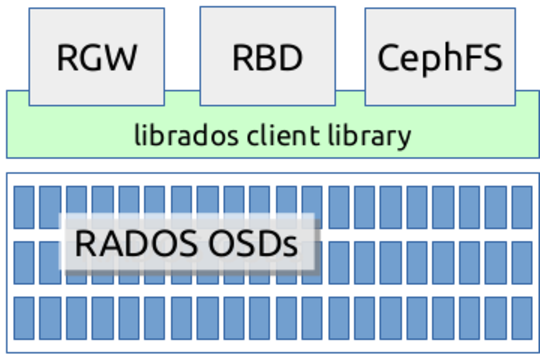
\includegraphics[width=1.0\linewidth]{figures/ceph}
      \caption{Ceph}
      \label{fig:ceph}
  \end{subfigure}\quad
  \begin{subfigure}[b]{.40\linewidth}
      \centering
      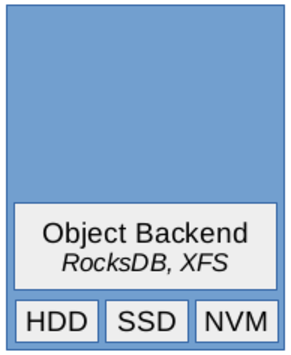
\includegraphics[width=1.0\linewidth]{figures/osd}
      \caption{OSD}
      \label{fig:osd}
  \end{subfigure}
  \caption{Ceph and OSD... gotta cram more stuff in here...}
\end{figure}

The object storage device (OSD), illustrated in Figure~\ref{fig:osd}, is the
building block of the RADOS cluster and is responsible for managing and
providing access to a set of
named objects. The configuration of an OSD is flexible, and commonly contains
a mix of commodity hardware such as HDD and SSD bulk storage, a multi-core
CPU, GBs of RAM, and one or two 10 Gb Ethernet links. Clients access object
data managed by an OSD by invoking object operations exposed by the OSD
such as reading or writing bytes, as well as more complex operations like taking
snapshots or composing one or more native operations into compound procedures
that execute in a transactional context.

The native object operations in RADOS roughly fall into two categories based
on the type of data being accessed: key-value items, or bulk bytestream data.
The key-value interface operates as a dedicated database associated with each
object, and the bytestream interface supports random byte-level access.  At a
low-level each of these abstract I/O interfaces map to hardware storage
devices through a pluggable object backend storage service. For instance,
LevelDB or RocksDB may be used to store key-value data, while the
\emph{FileStore} implementation maps the bytestream interface onto a local
POSIX file system~\cite{leveldb,rocksdb}. Several backend implementations
exist for storing data in targets such as a Kinetic Drive or in NVMe devices,
among others.

%Independent of the hardware or backends chosen, Ceph allows all
%object operations to be combined to create compound operations such as storing
%key-value metadata associated with a binary blob, allowing applications to
%build object interfaces that work even as Ceph software and hardware evolve.

\paragraph*{Object Classes}
While Ceph provides a wide variety of native object operations, it also
includes a facility referred to as \emph{object classes} that allow developers
to create application-specific object operations in the form of C++ shared
libraries dynamically loaded into the OSD process at runtime.  Object classes
can be used to implement basic data management tasks such as indexing
metadata, or used to perform complex operations such as data transformations
or filtering. Table~\ref{tab:objclass-cats} summarizes the range of object
classes maintained in the upstream Ceph project which support internal Ceph
subsystems as well as applications and services that run on top of Ceph.

\begin{table}[ht]
\centering
\begin{tabularx}{\columnwidth}{|X|l|l|l|}
\hline
Category & Specialization & Methods \\ \hline
\multirow{2}{*}{Locking} & Shared & \multirow{2}{*}{6} \\
                         & Exclusive & \\ \hline
\multirow{3}{*}{Logging} & Replica & 3 \\
                         & State & 4 \\
                         & Timestamped & 4 \\ \hline
Garbage Collection & Ref. Counting & 4 \\ \hline
\multirow{4}{*}{Metadata} & RBD & 37 \\
 & RGW & 27 \\
 & User & 5 \\
 & Version & 5 \\ \hline
\end{tabularx}
\caption{A variety of RADOS object storage classes exist that expose reusable
interfaces to applications.}
\label{tab:objclass-cats}
\end{table}

A critical step in the development of application-specific object interfaces
is deciding how to best make use of the native object interfaces. For instance
if an application stores an image in an object, it may also extract and store
EXIF metadata as key-value pairs in the object key-value database.  However,
depending on the application needs it may be sufficient or offer a performance
advantage to store this metadata as a header within the bytestream. In the remainder
of this section we will explore the challenges associated with these design questions.

\subsection{Motivating Application: CORFU}

The primary motivating example we will use in this paper is the CORFU
distributed shared-log designed to provide high-performance serialization
across a set of flash storage devices~\cite{balakrishnan:nsdi12}. The
shared-log is a powerful abstraction useful when building distributed systems
and applications, but common implementations such as Paxos or Raft funnel I/O
through a single node limiting the throughput of log
operations~\cite{lamport:tocs89}. The CORFU protocol addresses this limitation
by de-coupling log entry storage from log metadata management, making use of a
centeralized, volatile, in-memory \emph{sequencer service} that assigns log
positions to clients that are appending to the log. Since the sequencer is
centeralized serialization is trivial, and the use of non-durable state allows
the sequencer service to operate at very high rates. The CORFU system has been
used to demonstrate a number of interesting services such as transactional
key-value and metadata services, replicated state machines, and an elastic
cloud-based database management system~\cite{balakrishnan:sosp13,bernstein:cidr11}.

Two aspects of CORFU make its design attractive in the context of the Ceph
storage system. First, CORFU assumes a cluster of flash devices because
log-centric systems tend to have a larger percentage of random reads making it
difficult to achieve high-performance with spinning disks. However, the speed
of the underlying storage does not affect correctness. Thus, in a
software-defined storage system such as Ceph a single implementation can
transparently take advantage of any software or hardware upgrades, and make use
of existing and future data management features such as tiering in RADOS,
allowing users to freely choose between media types such as SSD, spinning
disks, or emerging NVRAM technologies.

\paragraph*{CORFU and Storage Programmability}
The second property of CORFU relevant in the context of Ceph is the dependency
CORFU places on custom storage device interfaces used to guarantee
serialization during failure and reconfiguration. Each flash device in a CORFU
cluster exposes a 64-bit write-once address space consisting of the primary I/O
interfaces \emph{write(pos, data)} and \emph{read(pos)} for accessing log
entries, as well as \emph{fill(pos)} and \emph{trim(pos)} that invalidate and
reclaim log entries, respectively. All I/O operations in CORFU initiated by
clients are tagged with an \emph{epoch} value, and flash devices are expected
to reject client requests that contian an old epoch value. To facilitate
recovery or handle system reconfiguration in CORFU, the storage devices are
also required to support a \emph{seal(epoch)} command that marks the latest
epoch and returns the maximum position written to that device. The seal
interface is used following the failure of a sequencer to calculate the tail of
the log that the sequencer should use to repopulate its in-memory state.

While the authors of the CORFU paper describe prototype device interfaces using
both host-based and FPGA-based implementations, RADOS \emph{directly} supports
the creation of logical storage devices through its object class feature
described previously in Section~\ref{sec:objclass}. Thus, by using
software-based object interfaces offered by RADOS flash devices in CORFU can be
replaced by software-defined storage offering significant flexibility and a
simplified design.

The implementation of a custom object class that satisifies the needs of an
application such as CORFU is often straightforward. However, as described in
Section~\ref{sec:objclass} there are a variety of native object I/O interfaces
available, and it is not always immediately clear how best to utilize these
interfaces. A common approach is to first define the set of requirements for
the desired interface, construct a design space parameterized on the set of
native interfaces, and winnow this space down through a process of elimination.

\paragraph*{Towards a CORFU Object Interface}
The state-machine shown in Figure~\ref{fig:corfu-sm} shows the composition of
actions for each component of the CORFU interface. For instance, all operations
begin by applying an \emph{epoch guard} that ensures the request is tagged with
an up-to-date epoch value. The \emph{read} (R) and \emph{write} (W) operations
both proceed by (1) examining metadata associated with the target position, (2)
performing I/O to read or write the log entry, and in the case of a write, (3)
updates metadata for the target log position.

\begin{figure}[t]
\centering
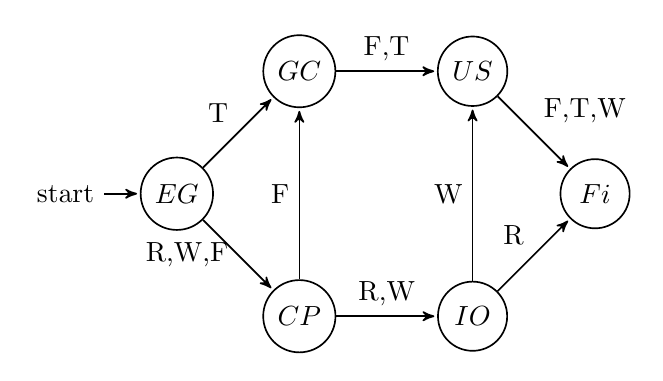
\begin{tikzpicture}[->,>=stealth',shorten >=1pt,auto,node distance=2.2cm,semithick]
%\tikzstyle{every state}=[fill=red,draw=none,text=white]

  \node[initial left,state] (A)              {$EG$};
  \node[state]         (B) [below right of=A] {$CP$};
  \node[state]         (D) [right of=B]       {$IO$};
  \node[state]         (C) [above right of=A] {$GC$};
  \node[state]         (E) [right of=C]       {$US$};
  \node[state]         (F) [below right of=E] {$Fi$};

  \path (A) edge        node [left] {R,W,F} (B)
            edge        node {T}     (C)
        (B) edge        node {F}     (C)
            edge        node {R,W}   (D)
        (C) edge        node {F,T}   (E)
        (D) edge        node {W}     (E)
            edge        node {R}     (F)
        (E) edge        node {F,T,W} (F);
\end{tikzpicture}
\caption{State transition diagram for read ($R$), write ($W$), fill ($F$), and
trim ($T$) CORFU operaitons. The states epoch guard ($EG$), check position ($CP$),
and update state ($US$) access metadata. The I/O performs a log entry read or
write, and garbage collection ($GC$) marks entries for reclamation.}
\label{fig:corfu-sm}
\end{figure}

The primary concern of an application developer when implementing an object
interface in Ceph is deciding how native interfaces are composed into a
compound operation. These types of decisions are commonly referred to as
physical design, and can affect performance and application flexibilty.
For instance, one valid design option is to store each log position in
an object with a name using a one-to-one mapping with the log entry position.
However, as we will see in the next section this choice of a physical design
can result in poor performance compared to other designs.

\subsection{Physical Design}

We categorize the challenges of physical design into log entry management, or
metadata management.

Our strategy is simply to construct the design space, and winnow it down using
a set of targetted experiments.

We'll start by forming a baseline performance profile without any protocol
overhead.

All designs store a log entry. We can benchmark the system without any
overhead associated with indexing or metadata management.

\paragraph*{Baseline Performance}

Figure~\ref{fig:pd-map} illustrates the two primary dimensions of the physical
design space. The first dimension concerns the strategy by which a log entry
is addressed within RADOS. In a one-to-one strategy each log entry is stored
in a distinct object with a name based on the log entry position.  This is an
attractive option because it is trivial for a client to address any log entry,
and an object interface does not require any complexity associated with
multiplexing multiple entries---addressing relies on native indexing provided
by the OSDs themselves. In contrast to a 1:1 strategy, an N:1 strategy
\emph{stripes} log entries across a smaller set of objects, introducing added
complexity into both the client and object interface implementations. The
second design dimension selects the primary storage interface for log
entries, namely the key-value or bytestream interfaces, described in
Section~\ref{sec:objclass}.

These two dimensions are represented by the first two columns of
Table~\ref{tab:pd-map} which describes the entire design space, where
\emph{KV} corresponds to the key-value interface, and the bytestream interface
is represented by \emph{AP} and \emph{EX} for an append or explicit i/o
straetgy.

. Note that we
decompose the bytestream I/O interface into two sub-strategies: I/O using
explicit offsets (EX), and appends (AP).

CORFU device interface requirements in Ceph as an object interface. So far we
have 


append is more attractive, all things being equal, as it supports flexible
mapping size.




There is a finite set of strategies for mapping the CORFU interfaces onto the
current set of native I/O interfaces used to construct object interfaces.
Table~\ref{tab:pd-map} shows the design space for mapping the CORFU interfaces
onto Ceph. In order to select the best mapping we performed a parameter sweet
over the design space.

\begin{figure*}[!ht]
    \centering
    \begin{subfigure}{.6\columnwidth}
        \includegraphics[width=\columnwidth]{experiments/librados-sweep/jewel_ssd.png}
        \caption{a}
        \label{fig:vanilla-io-diff}
    \end{subfigure}\hfill
    \begin{subfigure}{.6\columnwidth}
        \includegraphics[width=\columnwidth]{experiments/librados-sweep/firefly_ssd.png}
        \caption{b}
    \end{subfigure}\hfill
    \begin{subfigure}{.6\columnwidth}
        \includegraphics[width=\columnwidth]{experiments/basic-cls-overhead/output.1024.soft.reset.png}
        \caption{c}
    \end{subfigure}\hfill
    \caption{Shown here are the graphs and such that demonstrate that the same
        physical design choices are not the same between differing version of
    Ceph even on the same hardware.}
\end{figure*}

Figure~\ref{fig:vanilla-io-diff} shows the result of a parameter sweep which
clearly shows that an N-1 mapping based on the bytestream interface provides
superiour performance. However, the other two graphs show the same interfaces
running on an old version of Ceph that show the same decision would not have
been the optimal choice {\bf \emph{note: for the outline these are not the
real graphs we'll be using}}.

\begin{table}
\begin{tabular}{ | l | l | l | l | l |}
\hline
Map & I/O & Entry Size & Addressing & Metadata \\ \hline
\multirow{3}{*}{1:1} & KV  & Flex     & Ceph      & KV/BS \\ \cline{2-5}
                     & AP  & Flex     & Ceph/VFS  & KV/BS \\ \hline
\multirow{4}{*}{N:1} & KV  & Flex     & \multicolumn{2}{|c|}{KV/BS} \\ \cline{2-5}
                     & EX  & Fixed    & VFS       & KV/BS \\ \cline{2-5}
                     & AP  & Flex     & KV/BS     & KV/BS \\
\hline
\end{tabular}
\caption{The high-level design space of mapping CORFU log entry storage onto
the RADOS object storage system.}
\label{tab:pd-map}
\end{table}

\section{Programming Model}

In this section we are going to be describing our way of creating interfaces.

\section{Other Interfaces}

Here we show the derivation of two other interfaces that are in production in
Ceph today to demonstrate the generality of our interface.

\section{Evaluation}

\section{Related Work}

\section{Conclusion}

%In this section we examine the design space for implementing the CORFU
%protocol in the RADOS storage system. Table \ref{t:init-ds} shows the entire
%design space. A description of each design parameter follows:
%
%{\bf Mapping strategy.} The method by which a log entry---identified by its
%logical position---is addressed within RADOS is referred to as the mapping
%strategy. A 1:1 strategy stores each log entry in a RADOS object with a
%distinct name (e.g. ``mylog.pos443''), and an N:1 strategy stripes the log
%positions across a set of objects (e.g.  round-robin). While we do consider
%both strategies in this paper, a 1:1 strategy is attractive because it allows
%a design in which clients can directly address log positions by constructing
%the correct object name.
%
%{\bf Storage interface.} entry data may be small or large. its primary
%storage location is important. kv, bs. we further sub-divide bs into
%write and append. each strategy is compatible with fixed size entries
%except for the write interface.
%
%{\bf Logical addressing.}

%\subsection{Storage Interface Selection}
%
%Figure \ref{f:librados-sweep} shows the single-node write-only I/O throughput
%for each of the points in the design space defined in Table \ref{t:init-ds}.
%The results reveal poor relative performance using both the key-value storage
%interface, as well as either of the 1:1 strategies---which incur overhead by
%creating a new object for each log entry. Both of the N:1 strategies using the
%bytestream I/O interface outperform all of the other approaches by over 2x
%throughput, but otherwise have nearly identical performance.
%
%To examine the read performance of the points in the design space we generated
%a dataset using each of the write workloads, and then issued random reads
%across the entire dataset. Figure \ref{f:librados-rand-read} shows the read
%throughput for each of the design strategies. The results show that an N:1
%mapping using bytestream interface performs best. Interestingly, the 1:1
%mapping strategy using the bytestream interface exhibits good read performance
%in comparison to writes using the same strategy.

%\begin{figure}[h]
%  \centering
%  \includegraphics[width=0.45\textwidth]{experiments/librados-sweep/output.soft.reset.2hr.png}
%  \caption{
%[\href{https://github.com/noahdesu/zlog-popper/tree/master/experiments/librados-sweep/visualize.ipynb}{source}]
%Throughput (IOPS) of 1K writes to a single OSD using the standard I/O
%interfaces in various configurations. The best performance is achieved using
%the byte stream interface and a N:1 mapping strategy.
%}
%\end{figure}
%
%\begin{figure}[h]
%  \centering
%  \includegraphics[width=0.45\textwidth]{experiments/basic-cls-rand-read/output.read.60min.png}
%  \caption{
%[\href{https://github.com/noahdesu/zlog-popper/tree/master/experiments/basic-cls-rand-read/visualize.ipynb}{source}]
%Throughput of 1K random reads to a single OSD using the standard I/O
%interfaces in various configurations. The best performance is achieved using
%the byte stream interface and a N:1 mapping strategy.
%}
%\end{figure}
%
%\begin{figure}[h]
%  \centering
%  \includegraphics[width=0.45\textwidth]{experiments/basic-cls-overhead/output.1024.soft.reset.png}
%  \caption{
%[\href{https://github.com/noahdesu/zlog-popper/tree/master/experiments/basic-cls-overhead/visualize.ipynb}{source}]
%}
%\end{figure}


%As a first approximation these results show that when optimizing for log
%append and random read throughput the design space should be refined by
%limiting solutions to architectures based on a N:1 mapping strategy using the
%bytestream I/O interface. But what these microbenchmarks explicitly omit are
%the overheads associated with metadata management such as enforcing write-once
%semantics or using an index to map a log position to a physical offset within
%an object. In the next section we

\bibliography{paper}
\bibliographystyle{plain}

\end{document}
